\subsection{« Parler aux yeux » (Playfair) : de l’intérêt et des limites de la visualisation}\footnote{Expression empruntée au statisticien William Playfair, dans Eléments de statistique, Paris, 1802, cité dans \footcite{courtin_rapport_2019}}

Le Service numérique de la recherche de l’\inha, bien avant la mise en place du projet \pense, a développé ou commandité des projets de visualisation de données dans le cadre de la valorisation et de l’accompagnement de la recherche menée au sein de l’Institut. Citons parmi ces projets la visualisation sous forme de réseau réalisée dans le cadre du programme de recherche « Répertoire des acteurs du marché de l’art en France sous l’occupation » (RAMA)\footcite{inha_repertoire_nodate}, ou encore les cartographies interactives des données de la base RETIF (« Répertoire des tableaux italiens dans les collections publiques françaises ») \footcite{inha_repertoire_nodate-1}. 
Dans le cadre de \pense, la visualisation des données semble envisagée dès que les données s’y prêtent, soit en adoptant une approche « traditionnelle » de la datavisualisation, en empruntant des formes de modélisation bien établies (la cartographie avec le projet Thierry), soit en explorant des voies connexes, ancrées plutôt dans le design graphique, exploitant la matérialité du corpus pour en offrir une visualisation permettant d’en saisir l’aspect massif (\textit{Barye}) ou d’en restituer l’ambition ou la genèse intellectuelle (\textit{Karbowsky}). Pour toutes ces approches, diverses dans leurs objets et leurs héritages conceptuels, le \snr revendique ouvertement une démarche de  \textit{data storytelling}\footcite{inha_visualisation_nodate}, un concept qu’il peut a priori paraître étonnant de voir émerger dans le domaine des \shs, mais dont l’histoire est pourtant bien entrecroisée avec ces disciplines, notamment dans leur dimension quantitative.

\subsubsection{Recherche d’intelligibilité par la construction narrative : le data storytelling et son application par le SNR}

Le \textit{data storytelling}, ou narration de données, est un concept issu partiellement du monde de l’entreprise (avec notamment la notion voisine de \textit{business intelligence}) et du journalisme\footcite{sanders_developing_nodate}. La promesse du \textit{data storytelling} est de rendre intelligible des informations complexes à travers des représentations visuelles. Ce procédé est particulièrement pertinent dans un contexte où les chiffres et les analyses quantitatives sont souvent présentés de manière abstraite, rendant la compréhension difficile pour les non-initiés. La visualisation de données permet ainsi d’atténuer certains biais liés à une présentation exclusivement numérique des résultats, bien que certains inconvénients inhérents à cette approche méritent d’être discutés, notamment dans le domaine de la recherche scientifique. Nous y reviendrons plus tard.

Le \textit{data storytelling} peut être défini comme l’art de transformer des données brutes en une narration cohérente, rendant ainsi les informations non seulement compréhensibles, mais également exploitables. Comme le souligne \citeauthor{shao_data_2024}, cette pratique consiste à « tisser des faits, des insights, des émotions et des intentions dans une narration engageante qui imbue de sens des idées complexes » \footcite{shao_data_2024}. L’objectif est d’impliquer le public, de le pousser à réfléchir, voire à agir. En appliquant cette définition au domaine de la visualisation de données, le \textit{data storytelling} permet de donner vie aux données, les rendant accessibles et compréhensibles par un large public, tout en facilitant la prise de décision basée sur ces informations (d’où le lien avec la \textit{business intelligence} mentionnée plus haut).
\newline
\textbfit{Regard historique sur la visualisation de données}\\

Bien que le concept de \textit{data storytelling} apparaisse (et soit régulièrement marketé) comme une innovation récente, il s’inscrit dans une tradition plus ancienne de la visualisation des données. Dès les XVIIIème et XIXe siècles, les premiers praticiens de la statistique et de l’analyse de données ont compris l’importance de la présentation visuelle pour rendre intelligibles des questions complexes à un public non spécialisé. Kosara et MacKinlay (cités par  \citeauthor{shao_data_2024}) notent que ces premières tentatives de visualisation ressemblaient déjà aux pratiques actuelles du \textit{data storytelling}, leur objectif étant de montrer, d’expliquer ou de souligner l’ampleur de certains problèmes à des décideurs ou à des publics peu familiers des chiffres. La présentation visuelle ne doit pas se contenter de montrer des chiffres ; elle doit également donner du sens à ces chiffres et permettre de dégager des tendances claires et exploitables. Cette approche a profondément influencé le développement de la visualisation des données, tant dans le domaine scientifique que dans le domaine commercial\footcite{shao_data_2024}.

Le \textit{data storytelling} s’inscrit ainsi dans une histoire plus large de la visualisation des données, elle-même étroitement liée aux évolutions épistémologiques de la statistique. Lev Manovich, dans son analyse de l’histoire de la discipline, identifie trois phases marquantes\footcite[p.19-20]{manovich_data_2015}. 
La première phase, qui s’étend du XVIIIe siècle jusqu’à la première partie du XIXe siècle, est marquée par la collecte et la tabulation de données sociales et économiques. Durant cette période, des pionniers comme William Playfair développent des techniques graphiques de nos jours désormais incontournables, telles que le diagramme en barres, le graphique en courbes, le diagramme circulaire et le graphique en secteurs. Ces premières tentatives ne permettaient cependant de visualiser qu’une seule dimension des objets étudiés, limitant ainsi la portée analytique des représentations.
La deuxième phase, entre les années 1830 et 1890, voit l’apparition de techniques « analytiques et graphiques » permettant d’étudier les relations entre les phénomènes. L’introduction des concepts de corrélation et de régression à la fin du XIXème engendre l’utilisation du diagramme de dispersion, ou \textit{scatterplot}, pour représenter graphiquement ces relations. Cette étape marque une avancée significative dans l’utilisation de la statistique pour visualiser les liens entre différents ensembles de données.
Enfin, la troisième phase, s’étendant de 1900 à 1930, est caractérisée par la systématisation et l’extension des concepts statistiques, notamment grâce aux travaux de Karl Pearson, Charles Spearman, Ronald Fisher et Charles Pierce. Ces chercheurs ont raffiné les concepts tels que la moyenne et la médiane, et ont mis au point des méthodes pour analyser les relations entre deux variables. Cette phase marque la fondation de la statistique moderne, avec des outils et des concepts qui perdurent aujourd’hui dans les domaines de l’analyse quantitative et de la visualisation de données\footcite[p.19-20]{manovich_data_2015}. 

L’histoire de la visualisation de données est aussi marquée par son application dans le domaine de la santé publique, notamment pour représenter la propagation des épidémies. À partir du XVIIIe siècle, avec l’émergence des statistiques modernes, la visualisation devient un outil majeur pour comprendre les dynamiques des populations et de la santé et ainsi envisager de les prévenir et de les anticiper. John Snow au milieu du XIXème siècle, par exemple, utilisa une superposition cartographique pour retracer les sources de l’épidémie de choléra à Londres (et ainsi tenter de l’enrayer), tandis que Florence Nightingale employa des diagrammes en rose pour illustrer les causes de la surmortalité des soldats de la Guerre de Crimée (et ainsi proposer des méthodes hygiéniques pour y remédier). Enfin, le \textit{diagramme de Sankey} de Charles Joseph Minard, retraçant l’émiettement de l’armée napoléonienne lors de la Retraite de Russie, est aujourd’hui considéré comme l’une des visualisations de données les plus emblématiques « de tous les temps », comme le remarque Elyse Graham\footcite[p.450]{graham_introduction_2017}.
Ces premiers « récits de données » visaient non seulement à illustrer l’ampleur de certaines crises sanitaires, mais également à sensibiliser voire à pousser les autorités à agir, comme l’ont relevé, entre autres\footnote{Voir à ce sujet le rôle de la visualisation cartographique dans la prise de conscience des inégalités liées à l’accès des populations non-blanches à l’eau potable dans un quartier du Midwest des Etats-Unis : \footcite{jeffries_how_2014}}, \citeauthor{shao_data_2024}.
\newline
\textbfit{Datavisualisation et SHS}\\

La visualisation de données, dont l’intégration dans les \shs n’est pas récente, ne relève pas toujours tout à fait du réflexe dans le domaine des humanités traditionnelles, en partie en raison du fait qu’elle est souvent (voire exclusivement, pour un certain nombre de représentations canoniques) associée au traitement de données quantitatives. Selon \citeauthor{pawlicka_data_2017}, la forte poussée vers l’intégration systématique des techniques de visualisation de données dans ces disciplines peut même être interprétée comme une tentative de « scientification » des humanités, visant à défendre leur financement en les rapprochant des sciences dures\footcite[p.526]{pawlicka_data_2017}, qui disposeraient, elles, du point de vue d’un certain côté de la société et l’échiquier politique, d’une forme de légitimité à s’établir comme « véritables sciences ». Selon plusieurs auteurs, la démarche adoptée par la datavisualisation, lorsqu’implantée systématiquement, cherche à présenter des résultats empiriques dans un format qui, bien que visuellement convaincant, ne correspond pas toujours à la nature des recherches en sciences humaines, où la complexité et la multiplicité des interprétations doivent être prises en compte. Comme nous le verrons plus loin, la datavisualisation constitue bien une médiation, une interprétation de l’information à part entière, et non une simple représentation factuelle.  

Cependant, en dépit de ces critiques relatives aux biais inhérents à la représentation interprétée de la donnée et à une dimension quantitative qui a pu historiquement inspirée de la méfiance dans le domaine des humanités traditionnelle, il est légitime de constater que la force du data storytelling et de la data visualisation en général réside avant tout dans sa capacité à rendre les données plus intelligibles et plus attractives pour un large public, permettant ainsi de capter l’attention du récepteur. Une visualisation bien conçue peut ainsi rendre explicite une information souvent noyée dans des discours scientifiques difficiles d’accès\footcite{shao_data_2024}.
\newline
\textbfit{Rendre intelligible l’information complexe}\\

La relation entre la visualisation et la cognition humaine n’est pas nouvelle. Plusieurs auteurs\footnote{Parmi lesquels \footcite[p.451]{graham_introduction_2017} et \footcite[p.536]{pawlicka_data_2017}} mettent en avant une donnée anatomique qui expliquerait le succès de la visualisation de données : près de « 30\% du cortex humain est dédié au traitement des informations visuelles », expliquant le rôle donné à la visualisation de la transmission et l’acquisition de la connaissance.    Son efficacité réside dans leur capacité à transformer des données abstraites en récits visuels engageants, en introduisant une véritable « médiation » \footcite[p.80-99]{hinrichs_defense_2019} (au sens proche de celui de vulgarisation), facilitant ainsi la compréhension et la prise de décision.
\newline
\textbfit{Choix de datavisualisation dans le cadre du projet PENSE}\\

Dans le cadre du projet \pense, plusieurs choix de datavisualisation ont été faits pour illustrer et rendre accessible l’édition numérique des lettres échangées entre Jacques Doucet et son bibliothécaire René-Jean. Ces choix sont justifiés par la volonté de mettre en avant les différents événements de la vie de Doucet, de ses collections et des relations épistolaires qu’il entretenait, tout en fournissant un accès direct aux lettres et aux informations pertinentes.

Le premier outil développé est une chronologie interactive\footcite{noauthor_chronologie_nodate}, qui propose une visualisation permettant une mise en évidence de son processus de constitution de collections (achats, ventes, etc.), alignée sur des données biographiques.

\begin{figure}[h] 
\centering 
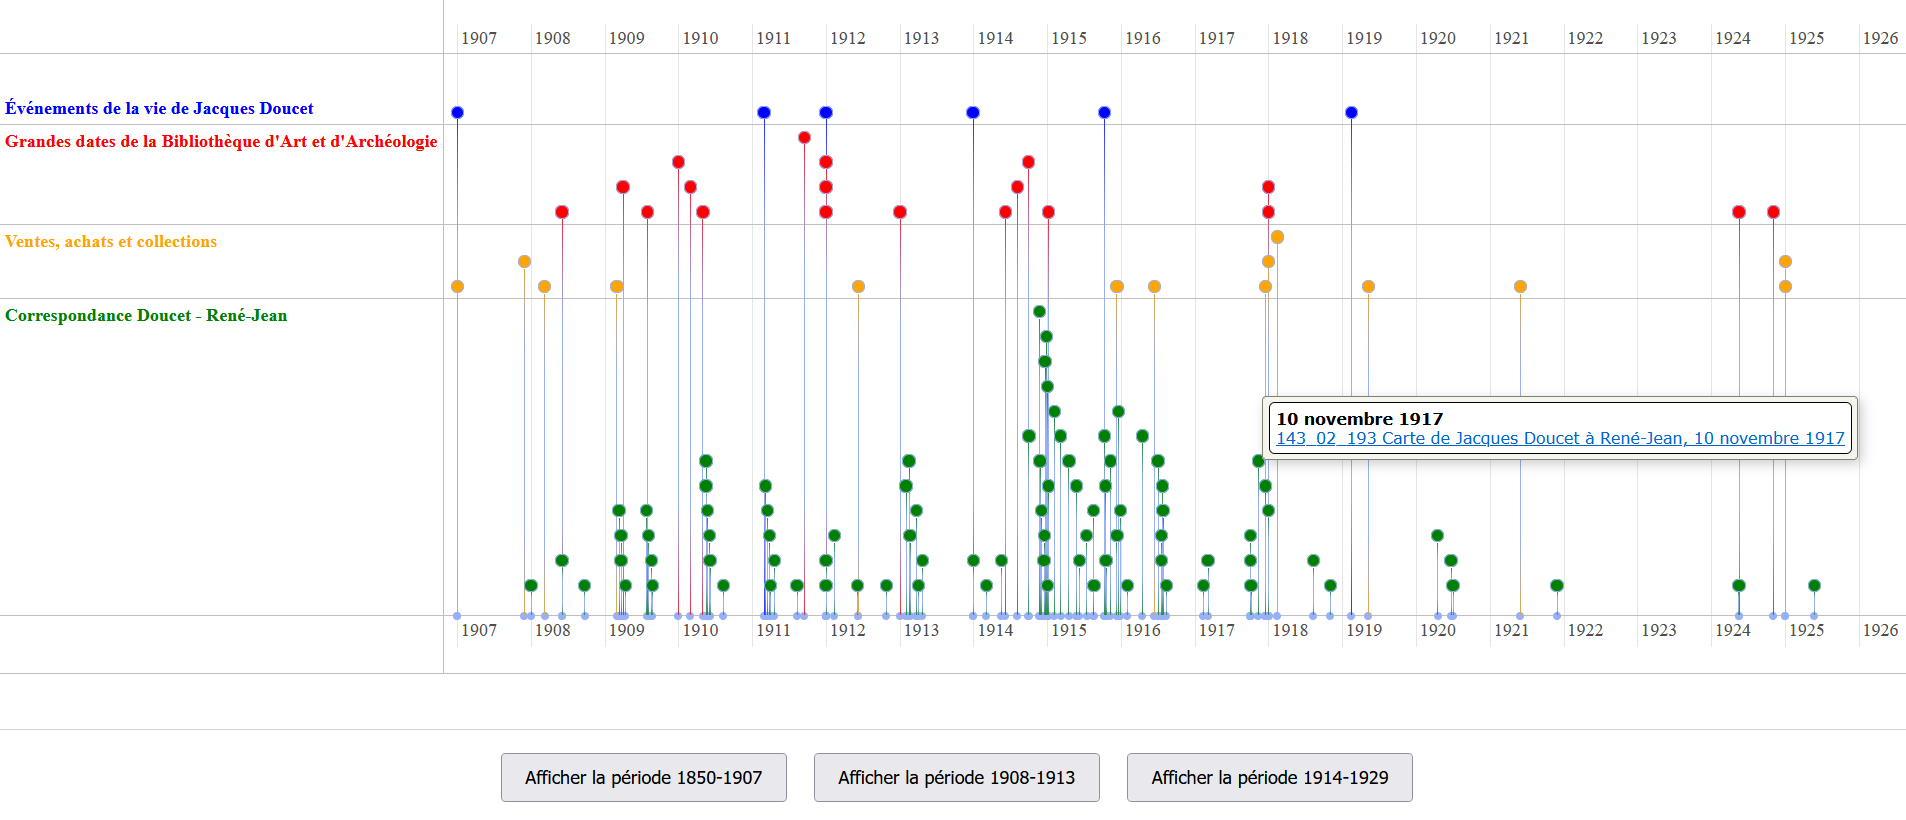
\includegraphics[width=0.8\textwidth]{chronologie} 
\caption{Prototype de chronologie interactive réalisée dans le cadre du stage pour le projet d’édition Doucet/René-Jean.} 
\label{fig:prototype-chrono} 
\end{figure}

Ce dispositif permet d'aligner sur une même ligne temporelle des dates relatives à des événements importants dans la vie de Doucet, les étapes principales de l'élaboration de la \baa, ainsi que la circulation des œuvres ayant appartenu à Doucet, le tout superposé sur la correspondance entretenue avec René-Jean, qui constitue l’arrière-plan principal de la visualisation. L’intérêt principal de cette chronologie réside dans sa capacité à synthétiser des données complexes sous une forme immédiatement lisible et accessible. Chaque événement est codé par une couleur spécifique permettant de distinguer facilement les catégories (correspondance, acquisition, vente, etc.). En survolant les points de la frise, une fenêtre informative apparaît, proposant un court descriptif de l’événement, souvent accompagné d'une image jugée évocatrice afin de renforcer l’immersion et la compréhension. De plus, pour la partie dédiée à la correspondance, l’utilisateur peut accéder directement à chaque lettre d’un simple clic, facilitant ainsi la navigation et l’interaction avec les documents originaux. Ce choix de datavisualisation, au-delà de son efficacité visuelle, permet une interaction fluide et intuitive avec le corpus.

La deuxième visualisation développée dans le cadre du stage est de forme cartographique\footcite{noauthor_carte_nodate}.

\begin{figure}[h] 
\centering 
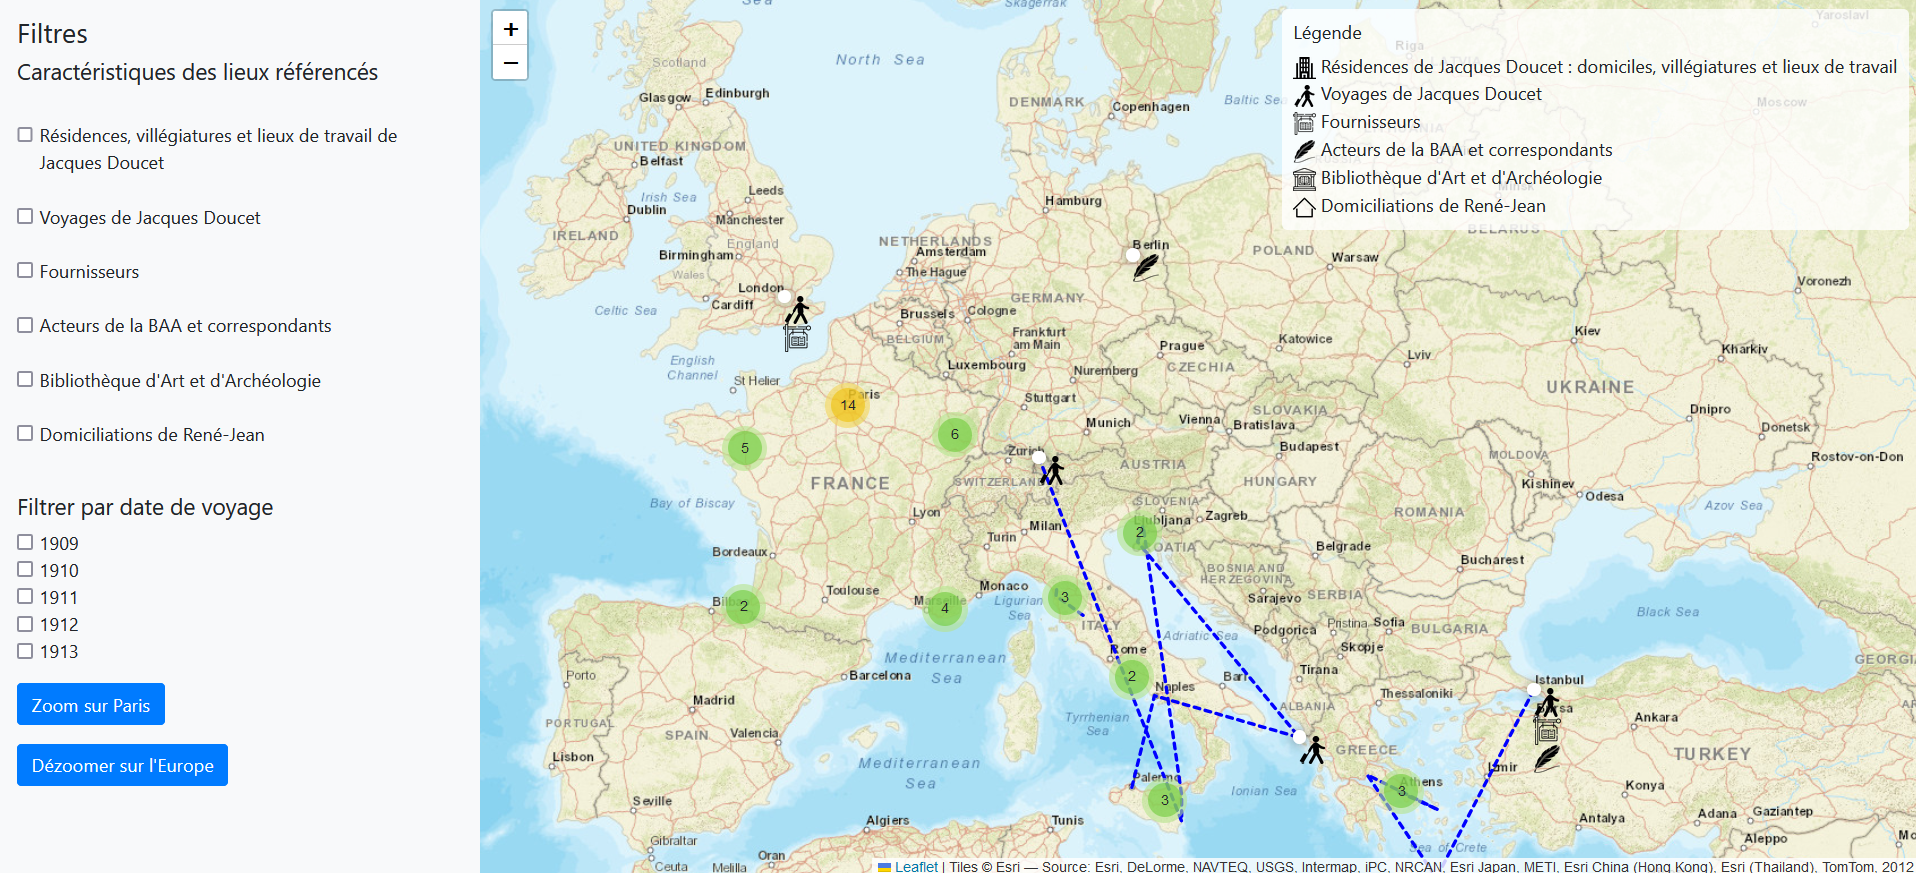
\includegraphics[width=0.8\textwidth]{cartographie} 
\caption{Prototype de cartographie interactive réalisée dans le cadre du stage pour le projet d’édition Doucet/René-Jean.} 
\label{fig:prototype-carto} 
\end{figure}

Cet outil permet de localiser géographiquement les lieux mentionnés dans la correspondance, qu’il s’agisse de résidences, d’étapes de voyages ou de localisations de fournisseurs et partenaires de Doucet. La carte est enrichie par des facettes de recherche permettant à l’utilisateur de filtrer les informations selon différents critères, tels que les résidences ou les voyages, ce qui facilite l'exploration des données spatiales du projet. 
Cette carte, en lien direct avec la correspondance, permet d’illustrer visuellement les réseaux de relations et d’échanges entretenus par Doucet à l’échelle internationale. Toutefois, elle est également soumise à des biais inhérents aux choix et contraintes technologiques et aux limites des sources. Par exemple, certains noms de personnes ou de lieux n’ont pas pu être inclus en raison de difficultés liées à l’identification ou à la qualité des sources, ce qui entraîne des lacunes dans la représentation des partenaires de Doucet sur la carte.

\subsubsection{La \textit{visual literacy} et la gestion des biais}

La datavisualisation est un outil puissant, mais elle comporte des limites importantes, notamment en ce qui concerne la manière dont elle est interprétée. La notion de \textit{visualisation literacy} (ou \textit{visual literacy}, selon les auteurs) met en lumière ces enjeux, en soulignant que même une visualisation bien conçue peut être mal comprise si le récepteur n’a pas les compétences nécessaires pour interpréter les données correctement. 
La \textit{visualisation literacy} est définie par \citeauthor{shao_data_2024} par la capacité à interpréter avec précision les représentations visuelles des données, et à extraire, traiter et tirer des conclusions à partir de celles-ci\footcite{shao_data_2024}. Cette compétence apparaît de nos jours comme une faculté critique dans une société où l’information visuelle (fondée ou non sur des données factuelles) circule abondamment, et où le recul à prendre face à ces représentations doit faire partie intégrante de l’apprentissage du citoyen\footcite[p.454]{graham_introduction_2017}.

Cependant, la responsabilité ne repose pas uniquement sur l’utilisateur, mais également sur le producteur des visualisations. C’est ici que la notion de biais entre en jeu, comme l’explique Johanna Drucker, qui propose de considérer les données non pas comme des faits objectifs existants par eux-mêmes indépendamment de tout contexte (« data »), mais comme des éléments construits et issus d’un travail d’interprétation et de reconceptualisation dans leur importation dans le milieu numérique (« capta »). Selon elle, les visualisations graphiques sont le produit d’un processus interprétatif, où chaque choix de représentation influe sur la manière dont les informations sont perçues. La distinction entre « data » et « capta », pour Drucker, renvoie à la différence fondamentale entre un savoir supposé objectif, « allant de soi », et une connaissance qui est en fait « manufacturée », construite et interprétée à partir de points de vue éminemment subjectifs\footcite[p.5]{drucker_humanities_2010}. En d’autres termes, créer une datavisualisation consiste à fabriquer du « capta » à partir de « capta », c’est-à-dire à prendre des éléments préexistants et à les organiser selon des structures qui sont elles-mêmes des « capta », conditionnées par des objectifs et des biais spécifiques. La transformation d’objets tels que le texte ou les œuvres d’art en données, phénomène voisin de celui décrit ici, est aussi critiquée chez Urzsula Pawlicka\footcite[p.531]{pawlicka_data_2017} comme comportant des risques d’effacement d’informations.
\newline
\textbfit{Quels biais à l’œuvre dans les prototypes de visualisation produits pour l’édition Doucet - René-Jean ?}\\

Dans le cadre des tâches de visualisation effectuées lors du stage, les choix de visualisation ont également été influencés par plusieurs facteurs techniques et théoriques, à commencer par les contraintes technologiques, temporelles et de compétences. 
Concernant la carte, par exemple, les outils utilisés, tels que la bibliothèque JavaScript Leaflet, ont offert des possibilités techniques importantes, notamment en termes d’ergonomie, de prise en main et d’interopérabilité (Leaflet étant la bibliothèque la plus fréquemment utilisée sur le Web pour la production de visualisations cartographiques), mais ces choix ont aussi imposé des contraintes. Le choix du fond de carte est l’un des principaux exemple de biais induit par un choix technologique, car il se base sur des représentations modernes qui ne correspondent pas toujours à la réalité historique des époques concernées. Le choix s’est porté sur un fonds de carte non vierge (contrairement à celui utilisé dans le cadre du projet Thierry par exemple) pour des raisons de compréhension, préférant invoquer à une représentation annotée (et familière) du monde, ce qui permet à l’utilisateur non spécialiste d’identifier rapidement les zones géographiques représentées. Cependant, le fonds de carte n’est pas historiquement juste, il ne correspond pas à la réalité géopolitique du monde tel que Doucet et René-Jean l’ont connu, ce qui constitue une lacune majeure.  L’idéal aurait été d’intégrer un fonds de carte correspondant à l’époque représentée, ce qui était possible techniquement en ayant recours à un fonds de carte d’atlas du début du XXème siècle libre de droit et accessible sur Gallica par exemple, combiné à un outil tel que QGIS pour la création cartographique. Cependant, en raison de contraintes tant technologiques (Leaflet étant plus facile d’accès) que temporelles, cette possibilité n’a pas été pleinement explorée. 
Par ailleurs, compte tenu des grands bouleversements géopolitiques ayant eu lieu sur la période couverte par la correspondance (1909-1928), un seul fonds de carte historique n’aurait pas constitué une visualisation complètement adéquate. On aurait pu envisager l’usage de plusieurs fonds de carte, organisés par tuilage, variant selon la période représentée, mais cela aurait soulevé des difficultés techniques et conceptuelles majeures, notamment en termes de cohérence de lisibilité des informations. 

D’autres biais ont pu émerger, et sont à signaler, dans la représentation des lieux ou des personnes. Certains noms de partenaires de Doucet, par exemple, n’ont pas pu être traités correctement en raison d’un traitement computationnel des sources qui n’a pu parvenir à saisir toutes les occurrences, notamment celles qui ne faisaient pas l’objet d’un balisage, ce qui conduit naturellement à des lacunes informationnelles dans la visualisation. 

Dans un autre domaine, les icônes utilisées dans la cartographie pour représenter certaines informations (résidences, voyages, correspondants, etc.) sont également sujettes à des biais culturels. La manière dont un lieu de villégiature ou un voyageur est représenté visuellement peut varier en fonction des conventions culturelles et graphiques, influençant ainsi la perception de ces informations. Nous nous sommes ici essentiellement basés sur une représentation occidentale contemporaine, fortement influencée par la signalétique commerciale notamment, en reprenant un style de pictogrammes que nous pourrions croiser dans notre vie quotidienne.

Dans le cas de la chronologie, il nous faut remarquer que notre visualisation a été fortement influencée par le premier prototype réalisé pour le projet par l’ingénieur en charge, réalisé à partir de la bibliothèque Vis.js, une solution technologique choisie pour sa facilité d’accès et sa rapide prise en main.

\begin{figure}[h] 
\centering 
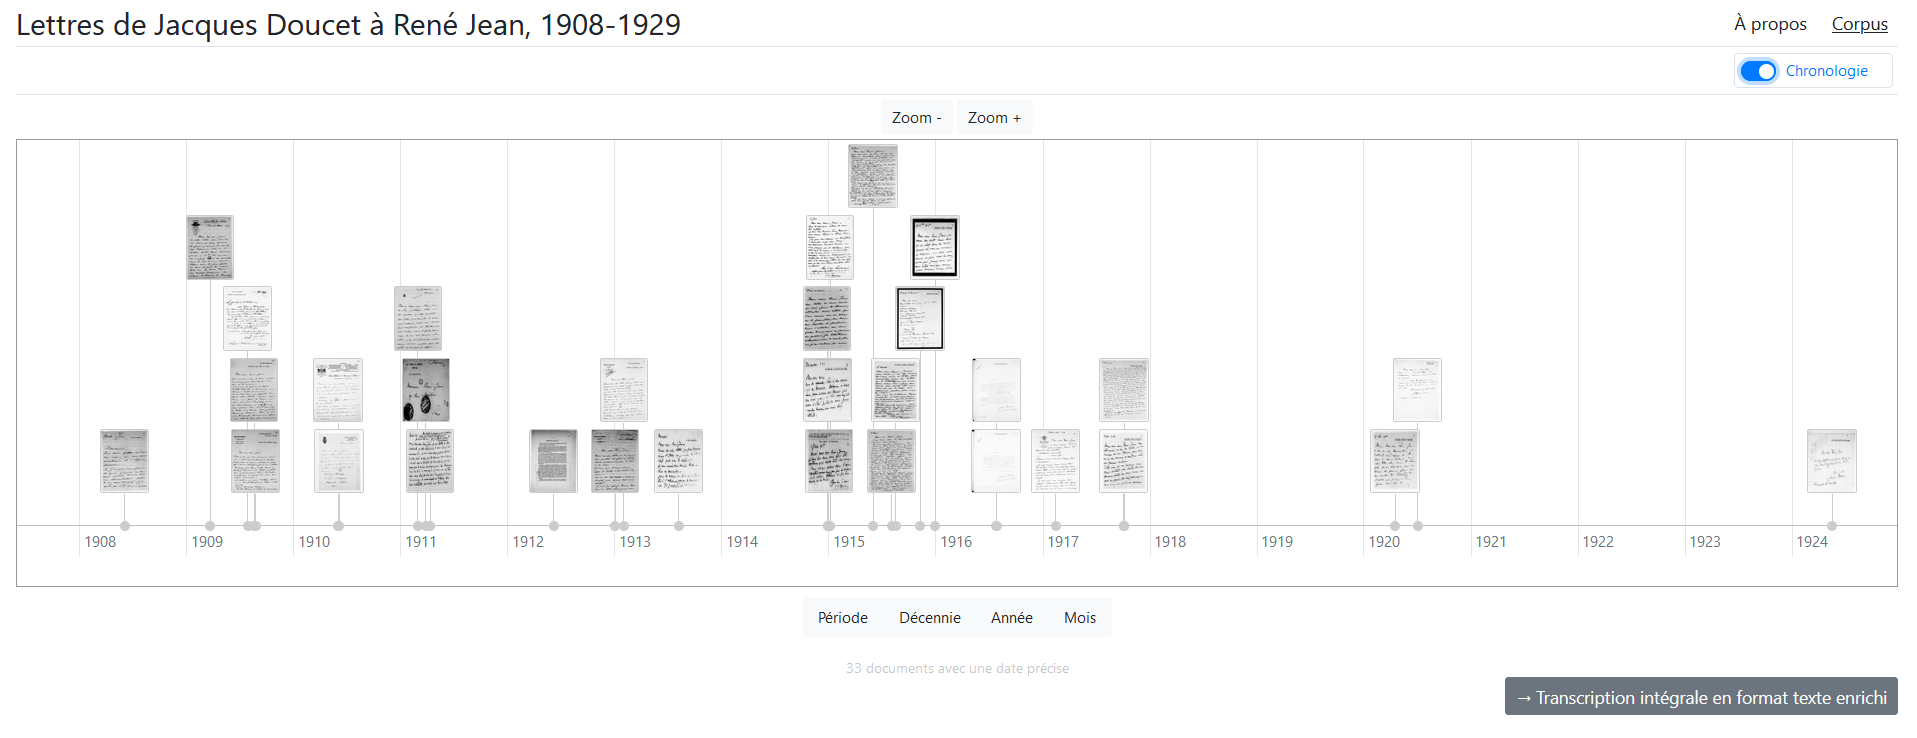
\includegraphics[width=0.8\textwidth]{prototype_prealable_chrono} 
\caption{Prototype de chronologie interactive réalisée par Jean-Christophe Carius pour le projet d’édition Doucet/René-Jean.} 
\label{fig:chrono-jcc} 
\end{figure}

Outre les aspects conditionnés par les contraintes particulière de cette solution logicielle (un « style » de visualisation relativement limité, une moins grande liberté offerte qu’avec D3.js, bibliothèque plus puissante mais moins accessible), certains biais semblent propres à la visualisation chronologique : choix des dates retenues, ce qui relève de la direction scientifique du projet, d’une part, et modélisation du temps, d’autre part (quel séquençage du temps opérer ? Un découpage par mois, par année ?). Nous avons privilégié une approche modulaire, permettant à l’utilisateur, par un système de zoom, de décider du point de focalisation de la chronologie : l’utilisateur peut ainsi techniquement zoomer jusqu’au niveau du jour individuel, les lettres étant associées à leur date précise (au jour près) de production. 

Ainsi, comme mis en évidence dans la présentation de nos choix, la datavisualisation, comme le souligne (entre autres) Johanna Drucker, n’est pas une simple représentation neutre de faits, mais le résultat d’un processus de sélection et d’interprétation où des choix et contraintes techniques et méthodologiques influencent directement le produit final.

\subsection{La datavisualisation comme partie intégrante du processus heuristique de recherche}

\subsubection{La datavisualisation comme « outil procédural » au centre de la philosophie de PENSE}

Dans la philosophie du projet \pense, la datavisualisation n’est pas seulement un outil de communication des résultats (comme elle pouvait peut-être l’être dans son acception initiale, chez Playfair par exemple), mais un véritable instrument heuristique au cœur du processus de recherche et de l’élaboration de la connaissance. Stalph et Heravi, cités par \citeauthor{sanders_developing_nodate} affirment que les datavisualisations remplissent à la fois une fonction épistémologique et une fonction communicative, il ne s’agit donc pas simplement de valoriser l’aboutissement d’une recherche, mais également de faire de la visualisation de données un nouveau point de départ pour de nouvelles analyses\footcite[p.6]{sanders_developing_nodate}, se rapprochant en cela de l’usage de la modélisation conceptuelle, permettant de poser un regard « neuf » sur les phénomènes étudiés. 
En ce sens, elles deviennent un véritable « outil procédural », intervenant dès la phase exploratoire, permettant de comprendre les données en cours de recherche, avant de les communiquer ensuite une fois les analyses terminées \footnote{\footcite[p.1645]{stalph_exploring_2021} cités par \footcite[p.6]{sanders_developing_nodate}}.     

Ce rôle central de la datavisualisation dans le processus de recherche se rapproche de la philosophie du \textit{design thinking}(\hyperlink{chap5}{voir chapitre 5}), où la modélisation visuelle est un moyen d’explorer des idées et de faire émerger de nouvelles perspectives. Dans le cadre de la mise en place des visualisations pour le projet \pense, cette démarche a été adoptée à travers un dialogue permanent entre les chercheurs et les développeurs, avec des prototypes visuels régulièrement mis à jour pour affiner les visualisations. Par exemple, les icônes et les appellations utilisées dans la cartographie ont fait l’objet de plusieurs reprises et révisions, illustrant le caractère itératif du processus. Cela souligne également l’idée que la datavisualisation n’est pas seulement une représentation finale, mais un élément central du processus d’élaboration de la connaissance.
La métaphore du château de sable, proposée par certains chercheurs\footcite{hinrichs_defense_2019}, illustre bien cette conception de la datavisualisation comme un processus dynamique et évolutif, où chaque visualisation est à la fois une « provocation esthétique » (cf. la dimension « attrayante » de la représentation visuelle de l’information), un « processus dynamique de questionnement » (cf. la dimension heuristique) et un « médiateur » pour la transmission efficace de l’information scientifique (cf. la dimension communicative). 